\section{Middleware}

O \textit{middleware} do subsistema, uma Raspberry, tinha como resultados
esperados uma aplicação que pudesse, ao rodar no embarcado, receber sinais e
enviá-los de maneira correta ao servidor.

Os resultados esperados foram atingidos. Foi desenvolvido a aplicação
Shoelace\footnote{\url{https://github.com/cadeiracuidadora/shoelace}}, que
serve como abstração para a aquisição dos dados do conversor A/D e que envia
os resultados para um servidor remoto.

Definimos que uma regra de negócio deveria ser que toda Raspberry tivesse
um \textit{token} e uma senha incluída, e esses dados são então utilizados nas
requisições para os servidores. Isso foi feito através da geração de dados
aleatórios (\textit{token} e senha), que são obtidos sempre que a Raspberry
é ligada, por estarem no \textit{bash\_rc}. Assim, todas as adições de sinais
feitas por uma dada Raspberry já serão relacionados com o respectivo paciente,
que poderá ter seus dados visualizados por parentes cadastrados.

A comunicação entre a Raspberry e o conversor é feita através do pacote em
Python \textbf{Adafruit\_ADS}, capaz de ler de até quatro canais ao mesmo tempo.
Contudo, uma ressalva: os valores enviados pelo sensor de temperatura não são
recebidos de uma maneira apresentável, por não estarem normalizados. Utilizamos
então a equação de Steinhart-hart:

$ 1/t = A + B * ln(R) + C[ln(R)]^3 $

Onde A, B e C são coeficientes, R é a resistência, e T a temperatura que
desejamos apresentar. Utilizamos os seguintes valores para os coeficientes:

$ A = 0.001129148; B = 0.000234125 ; C =  0.0000000876741 $

Para o cálculo do \textit{ln} utilizamos a função \textit{log1p} do Python, e
ressaltamos que tivemos diversos problemas de precisão, pois o Python arredonda
os resultados das operações de maneira grosseira em diversas situações. Por
fim, ajustamos outros parâmetros (como os utilizados na conversão da
resistência) utilizando outros resultados como base, de maneira experimental.

\subsection{Arquitetura}

A arquitetura do Shoelace foi feita pensando-se principalmente na
\textbf{extensão}. Desenvolvemos então essa aplicação de modo que, caso novos
sensores dos mais diversos tipos precisem ser utilizados, a adaptação no código
da Raspberry é simples. Uma classe abstrata \textbf{Sensor} força a implementação
do limiar referente ao sensor, e trás consigo funções que serão úteis, como o
cálculo da diferença percentual entre o valor enviado para o servidor e o valor
que está sendo analisado. A implementação de um novo sensor deve então
sobrescrever somente dois métodos: (i) o método \textit{limiar}, que diz qual a
diferença mínima entre o último valor enviado e um novo valor para que seja
enviado (útil na diminuição de sobrecarga do servidor, dificultando cenários de
\textit{backpressure}); e (ii) o método \textit{push\_callback}, que dá para o
sensor a liberdade de decidir o que fazer quando o limiar definido for atingido.
É nesse \textit{callback} que fazemos a requisição no servidor remoto.

\begin{figure}
    \begin{center}
        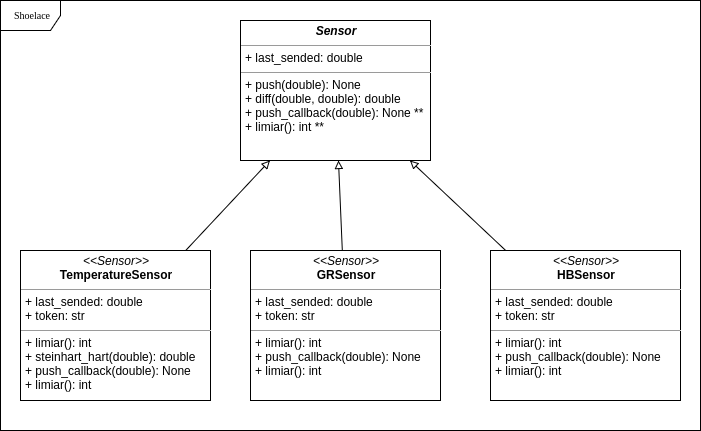
\includegraphics[scale=0.5]{figuras/shoelace.png}
    \end{center}
    \caption{Diagrama de classes do Shoelace. Métodos marcados com ** são
    abstratos.}
    \label{fig:shoelace}
\end{figure}

A Figura \ref{fig:shoelace} apresenta a arquitetura geral do Shoelace. É
ilustrado a implementação dos três sensores que utilizamos, mas caso novos
sensores precisem ser usados, basta criar uma classe que herde de Sensor, e
implementar os métodos necessários (\textit{limiar} e \textit{push\_callback}).
